%!TEX root = main.tex
\section{Design Guidelines\label{sec:guidelines}}
\subsection{Search-Browse Paradigm}
\subsection{Top-down approaches}
\subsection{Bottom-up approaches}

\begin{figure*}[ht!]
\centering
\vspace{-15pt}
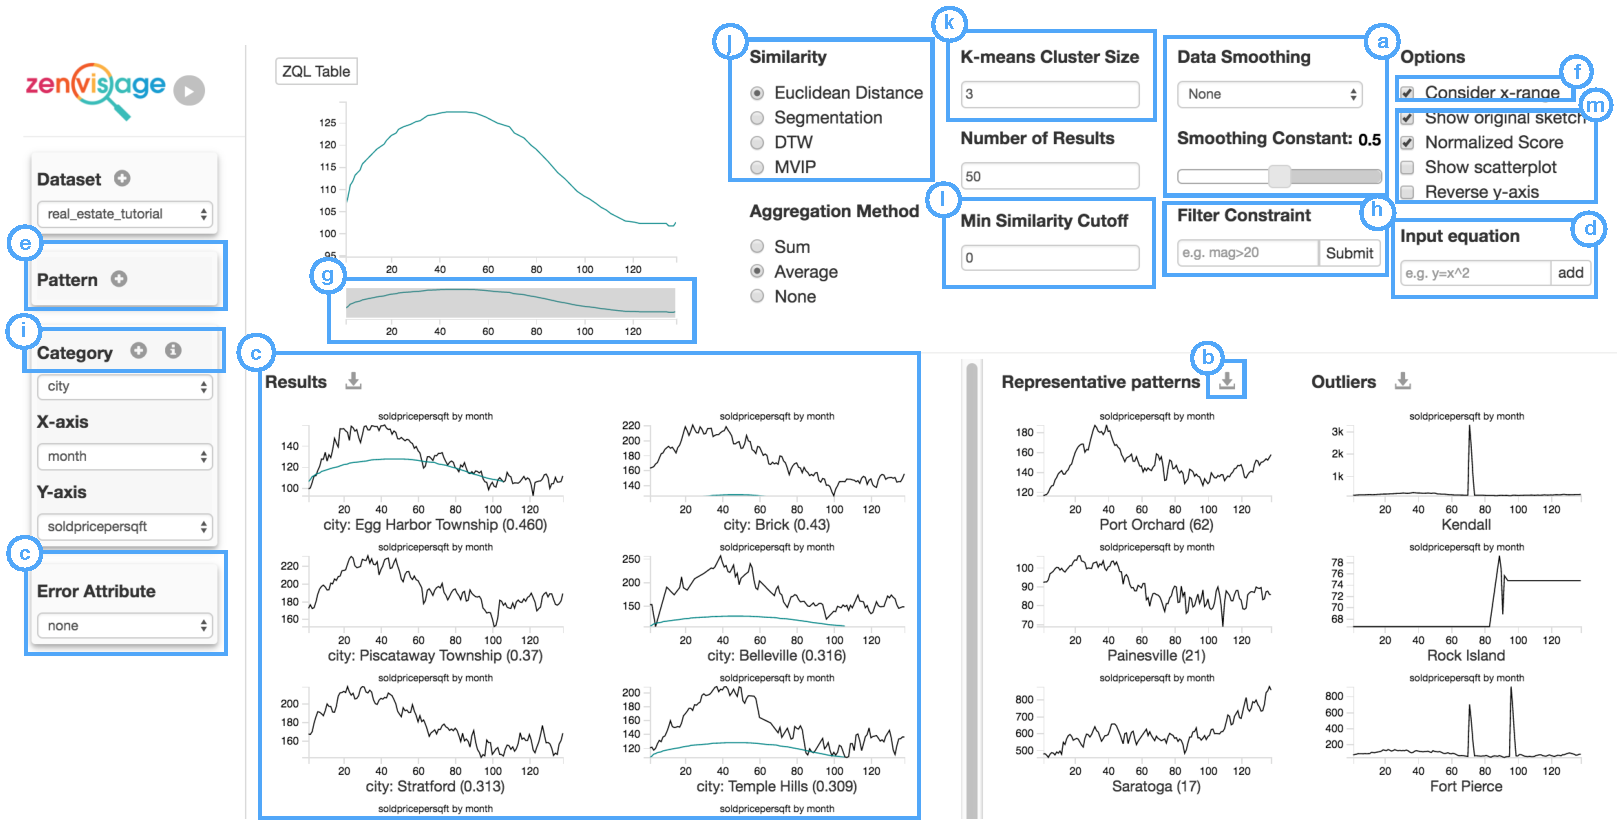
\includegraphics[width=\linewidth]{figures/newZV.pdf} %5.5
\vspace{-5pt}\caption{Our VQS after participatory design, which includes: the ability to preprocess via (a) interactive smoothing; (b, c) the ability to export data outputs ; querying functionalities via (d) equations and (e) patterns; query specification mechanisms including (f) x-range invariance, (g) x-range selection and filtering, (h) Filtering, and (i) Dynamic class creation; (j, k, l) system parameter options; (m) visualization display options. Prior to the participatory design, \zv only included a single sketch input with no additional options. \zv also displayed representative patterns and outlier patterns, as shown in Figure~\ref{oldZV}.}
\label{zvOverview}
\vspace{-14pt}
\end{figure*}